\begin{pastexam}[label={px:nsysu-112-osds-03}]{中山資工所甲組 112 學年度 第 3 題}
（計算）

(10\%) Suppose that there are 6 data elements $A, B, C, D, E, F$ with their searching frequencies 4, 9,
1, 6, 8, 7, respectively, where $A<B<C<D<E<F$. Please present the optimal binary search tree built with
these 6 elements such that the searching cost is minimized.
\end{pastexam}

\begin{pastsoln}
答案：根是 $E$；$E$ 的左子 $B$、右子 $F$；$B$ 的左子 $A$、右子 $D$；$D$ 的左子 $C$。 搜尋成本
（頻率乘以所在層數的和）$74$，最佳樹只有這一棵。

題目只給成功搜尋的頻率，沒有失敗搜尋（虛擬鍵）的頻率，所以成本定義成
$\sum_k f_k \cdot \text{depth}(k)$，根的深度算 $1$，也就是總比較次數。 這是資結書第~18.4~節的最佳
二元搜尋樹去掉虛擬鍵（$q_i = 0$）的情形。

\textbf{遞迴式}。 把鍵依序編成 $1..6$（$A..F$）。 令 $c(i, j)$ 是用第 $i$ 到第 $j$ 個鍵建出的最佳子樹的
成本，$W(i, j) = f_i + \cdots + f_j$。 選 $r$ 當根，左右子樹裡每個鍵都下降一層，多出 $W(i, j) - f_r$，
加上根自己的 $f_r$，總共多 $W(i, j)$：
\[
c(i, j) = W(i, j) + \min_{i \le r \le j} \bigl(c(i, r-1) + c(r+1, j)\bigr), \qquad c(i, i-1) = 0.
\]

\textbf{依長度填表}。 每格寫成「$c$（根）」；列出各候選根的值，方便核對。
\begin{center}
\small
\begin{tabular}{lcl}
\toprule
區間 & $W$ & 各根的 $c(i, r-1) + c(r+1, j) + W$ \quad $\Rightarrow$ $c$（根） \\
\midrule
單一鍵 & & $A{:}\,4$，$B{:}\,9$，$C{:}\,1$，$D{:}\,6$，$E{:}\,8$，$F{:}\,7$ \\
$A..B$ & 13 & $A{:}\,22$，$B{:}\,17$ \quad $\Rightarrow$ $17$（$B$） \\
$B..C$ & 10 & $B{:}\,11$，$C{:}\,19$ \quad $\Rightarrow$ $11$（$B$） \\
$C..D$ & 7 & $C{:}\,13$，$D{:}\,8$ \quad $\Rightarrow$ $8$（$D$） \\
$D..E$ & 14 & $D{:}\,22$，$E{:}\,20$ \quad $\Rightarrow$ $20$（$E$） \\
$E..F$ & 15 & $E{:}\,22$，$F{:}\,23$ \quad $\Rightarrow$ $22$（$E$） \\
$A..C$ & 14 & $A{:}\,25$，$B{:}\,19$，$C{:}\,31$ \quad $\Rightarrow$ $19$（$B$） \\
$B..D$ & 16 & $B{:}\,24$，$C{:}\,31$，$D{:}\,27$ \quad $\Rightarrow$ $24$（$B$） \\
$C..E$ & 15 & $C{:}\,35$，$D{:}\,24$，$E{:}\,23$ \quad $\Rightarrow$ $23$（$E$） \\
$D..F$ & 21 & $D{:}\,43$，$E{:}\,34$，$F{:}\,41$ \quad $\Rightarrow$ $34$（$E$） \\
$A..D$ & 20 & $A{:}\,44$，$B{:}\,32$，$C{:}\,43$，$D{:}\,39$ \quad $\Rightarrow$ $32$（$B$） \\
$B..E$ & 24 & $B{:}\,47$，$C{:}\,53$，$D{:}\,43$，$E{:}\,48$ \quad $\Rightarrow$ $43$（$D$） \\
$C..F$ & 22 & $C{:}\,56$，$D{:}\,45$，$E{:}\,37$，$F{:}\,45$ \quad $\Rightarrow$ $37$（$E$） \\
$A..E$ & 28 & $A{:}\,71$，$B{:}\,55$，$C{:}\,65$，$D{:}\,55$，$E{:}\,60$ \quad $\Rightarrow$ $55$（$B$ 或 $D$） \\
$B..F$ & 31 & $B{:}\,68$，$C{:}\,74$，$D{:}\,64$，$E{:}\,62$，$F{:}\,74$ \quad $\Rightarrow$ $62$（$E$） \\
$A..F$ & 35 & $A{:}\,97$，$B{:}\,76$，$C{:}\,86$，$D{:}\,76$，$E{:}\,74$，$F{:}\,90$ \quad $\Rightarrow$ $74$（$E$） \\
\bottomrule
\end{tabular}
\end{center}
例如 $A..F$ 取 $E$ 當根：$c(A..D) + c(F..F) + 35 = 32 + 7 + 35 = 74$。 $A..E$ 有兩個最佳根，但它不在最後
那棵樹的路徑上，不影響答案。

\textbf{回推樹}。 $A..F$ 的根 $E$，左邊 $A..D$、右邊 $F$。 $A..D$ 的根 $B$，左邊 $A$、右邊 $C..D$。
$C..D$ 的根 $D$，左邊 $C$。
\begin{center}
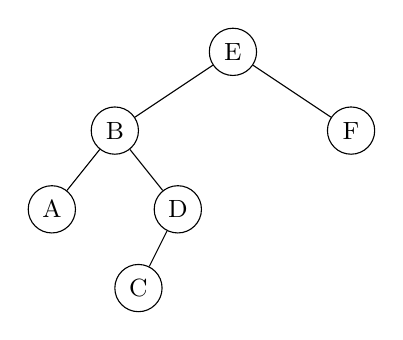
\begin{tikzpicture}[level distance=10mm,
  every node/.style={circle,draw,inner sep=1pt,minimum size=6mm,font=\small},
  level 1/.style={sibling distance=30mm}, level 2/.style={sibling distance=16mm},
  level 3/.style={sibling distance=10mm}]
\node {E}
  child {node {B}
    child {node {A}}
    child {node {D} child {node {C}} child[missing]}}
  child {node {F}};
\end{tikzpicture}
\end{center}
驗算成本：$E$ 在第 $1$ 層，$B, F$ 在第 $2$ 層，$A, D$ 在第 $3$ 層，$C$ 在第 $4$ 層：
$8 \cdot 1 + (9 + 7) \cdot 2 + (4 + 6) \cdot 3 + 1 \cdot 4 = 8 + 32 + 30 + 4 = 74$。 平均比較次數
$74/35 \approx 2.11$。
\end{pastsoln}
